\documentclass[11pt, onesided]{book}

%%%%%%%%%%%%%%Include Packages%%%%%%%%%%%%%%%%%%%%%%%%%%
\usepackage{xcolor}
\usepackage{mathtools}
\usepackage[a4paper, total={6in, 8in}, margin=1.25in]{geometry}
\usepackage{amsmath}
\usepackage{amssymb}
\usepackage{paralist}
\usepackage{rsfso}
\usepackage{amsthm}
\usepackage{wasysym}
\usepackage[inline]{enumitem}   
\usepackage{hyperref}
\usepackage{tocloft}
\usepackage{wrapfig}
\usepackage{titlesec}
\usepackage{colortbl}
\usepackage{stackengine} 
%%%%%%%%%%%%%%%%%%%%%%%%%%%%%%%%%%%%%%%%%%%%%%%%%%%%%%%%


%%%%%%%%%%%%%%%Chapter Setting%%%%%%%%%%%%%%%%%%%%%%%%%%
\definecolor{gray75}{gray}{0.75}
\newcommand{\hsp}{\hspace{20pt}}
\titleformat{\chapter}[hang]{\Huge\bfseries}{\thechapter\hsp\textcolor{gray75}{$\mid$}\hsp}{0pt}{\Huge\bfseries}
%%%%%%%%%%%%%%%%%%%%%%%%%%%%%%%%%%%%%%%%%%%%%%%%%%%%%%%%

%%%%%%%%%%%%%%%%%Theorem environments%%%%%%%%%%%%%%%%%%%
\newtheoremstyle{break}
  {\topsep}{\topsep}%
  {\itshape}{}%
  {\bfseries}{}%
  {\newline}{}%
\theoremstyle{break}
\theoremstyle{break}
\newtheorem{axiom}{Axiom}
\newtheorem{thm}{Theorem}[section]
\renewcommand{\thethm}{\arabic{section}.\arabic{thm}}
\newtheorem{lem}{Lemma}[thm]
\newtheorem{cor}{Corollary}[thm]
\newtheorem{defn}{Definition}[thm]
\newenvironment{indEnv}[1][Proof]
  {\proof[#1]\leftskip=1cm\rightskip=1cm}
  {\endproof}
%%%%%%%%%%%%%%%%%%%%%%%%%%%%%%%%%%%%%%%%%%%%%%%%%%%%%%


%%%%%%%%%%%%%%%%%%%%%%%Integral%%%%%%%%%%%%%%%%%%%%%%%
\def\upint{\mathchoice%
    {\mkern13mu\overline{\vphantom{\intop}\mkern7mu}\mkern-20mu}%
    {\mkern7mu\overline{\vphantom{\intop}\mkern7mu}\mkern-14mu}%
    {\mkern7mu\overline{\vphantom{\intop}\mkern7mu}\mkern-14mu}%
    {\mkern7mu\overline{\vphantom{\intop}\mkern7mu}\mkern-14mu}%
  \int}
\def\lowint{\mkern3mu\underline{\vphantom{\intop}\mkern7mu}\mkern-10mu\int}
%%%%%%%%%%%%%%%%%%%%%%%%%%%%%%%%%%%%%%%%%%%%%%%%%%%%%%



\newcommand{\R}{\mathbb{R}}
\newcommand{\N}{\mathbb{N}}
\newcommand{\Z}{\mathbb{Z}}
\newcommand{\Q}{\mathbb{Q}}
\newcommand{\C}{\mathbb{C}}
\newcommand{\T}{\mathcal{T}}
\newcommand{\M}{\mathcal{M}}
\newcommand{\Symm}{\text{Symm}}
\newcommand{\Alt}{\text{Alt}}
\newcommand{\Int}{\text{Int}}
\newcommand{\Bd}{\text{Bd}}
\newcommand{\Power}{\mathcal{P}}
\newcommand{\ee}[1]{\cdot 10^{#1}}
\newcommand{\spa}{\text{span}}
\newcommand{\sgn}{\text{sgn}}
\newcommand{\degr}{\text{deg}}
\newcommand{\pd}{\partial}
\newcommand{\that}[1]{\widetilde{#1}}
\newcommand{\lr}[1]{\left(#1\right)}
\newcommand{\vmat}[1]{\begin{vmatrix} #1 \end{vmatrix}}
\newcommand{\bmat}[1]{\begin{bmatrix} #1 \end{bmatrix}}
\newcommand{\pmat}[1]{\begin{pmatrix} #1 \end{pmatrix}}
\newcommand{\rref}{\xrightarrow{\text{row\ reduce}}}
\newcommand{\txtarrow}[1]{\xrightarrow{\text{#1}}}
\newcommand\oast{\stackMath\mathbin{\stackinset{c}{0ex}{c}{0ex}{\ast}{\Circle}}}
\newcommand{\txt}{Wald's \textit{General Relativity}}

\newcommand{\note}{\color{red}Note: \color{black}}
\newcommand{\remark}{\color{blue}Remark: \color{black}}
\newcommand{\example}{\color{green}Example: \color{black}}
\newcommand{\exercise}{\color{green}Exercise: \color{black}}

%%%%%%%%%%%%%%%%%%%%%%Roman Number%%%%%%%%%%%%%%%%%%%%%%%
\makeatletter
\newcommand*{\rom}[1]{\expandafter\@slowromancap\romannumeral #1@}
\makeatother
%%%%%%%%%%%%%%%%%%%%%%%%%%%%%%%%%%%%%%%%%%%%%%%%%%%%%%%%%

%%%%%%%%%%%%%table of contents%%%%%%%%%%%%%%%%%%%%%%%%%%%%
%\setlength{\cftchapindent}{0em}
%\cftsetindents{section}{2em}{3em}
%
%\renewcommand\cfttoctitlefont{\hfill\huge\bfseries}
%\renewcommand\cftaftertoctitle{\hfill\mbox{}}
%
%\setcounter{tocdepth}{2}
%%%%%%%%%%%%%%%%%%%%%%%%%%%%%%%%%%%%%%%%%%%%%%%%%%%%%%%%%%


%%%%%%%%%%%%%%%%%%%%%Footnotes%%%%%%%%%%%%%%%%%%%%%%%%%%%
\newcommand\blfootnote[1]{%
  \begingroup
  \renewcommand\thefootnote{}\footnote{#1}%
  \addtocounter{footnote}{-1}%
  \endgroup
}
%%%%%%%%%%%%%%%%%%%%%%%%%%%%%%%%%%%%%%%%%%%%%%%%%%%%%%%%%

%%%%%%%%%%%%%%%%%%%%%Section%%%%%%%%%%%%%%%%%%%%%%%%%%%%%
\makeatletter
\def\@seccntformat#1{%
  \expandafter\ifx\csname c@#1\endcsname\c@section\else
  \csname the#1\endcsname\quad
  \fi}
\makeatother
%%%%%%%%%%%%%%%%%%%%%%%%%%%%%%%%%%%%%%%%%%%%%%%%%%%%%%%%%

%%%%%%%%%%%%%%%%%%%%%%%%%%%%%%%%%%%Enumerate%%%%%%%%%%%%%%
\makeatletter
% This command ignores the optional argument 
% for itemize and enumerate lists
\newcommand{\inlineitem}[1][]{%
\ifnum\enit@type=\tw@
    {\descriptionlabel{#1}}
  \hspace{\labelsep}%
\else
  \ifnum\enit@type=\z@
       \refstepcounter{\@listctr}\fi
    \quad\@itemlabel\hspace{\labelsep}%
\fi}
\makeatother
\parindent=0pt
%%%%%%%%%%%%%%%%%%%%%%%%%%%%%%%%%%%%%%%%%%%%%%%%%%%%%%%%%%



\begin{document}

	\begin{titlepage}
		\begin{center}
			\vspace*{0.5cm}
			\Huge \color{red}
				\textbf{Reading Notes}\\
			\vspace{0.5cm}			
			\Large \color{black}
			\textit{General Relativity} by Robert Wald\\
			\vspace{1.5cm}

			
\includegraphics[scale=1.15]{hmm.pdf}
			
			
			\vspace{2cm}
			\LARGE
				\textbf{Jinyan Miao}\\
				\hfill\break
				\LARGE Winter 2023\\
			\vspace{1cm}

		\vspace*{\fill}
		\end{center}			
	\end{titlepage}



\tableofcontents
\hfill\break
\hfill\break
\hfill\break
 


\newpage
\chapter{The Spacetime Model}
\section*{Chapter 1 - 3 on Wald's \textit{General Relativity}}
These chapters on the book introduce the basic mathematical model used in general relativity. We start with the intuition of the spacetime metric, then we explore Lorentzian manifolds, curvatures, and geodesics in a manner similar to Riemannian geometry. 
\hfill\break
\hfill\break


\section[Modeling Spacetime using Manifolds and Metric Tensors]{\color{red}Modeling Spacetime using Manifolds and Metric Tensors\color{black}}
The word \textit{spacetime} in relativity theory refers to a continuum composed of \textit{events}. Each event is thought of as a point in \textit{space} at an instant of \textit{time}. Consider living in a $3$-dimensional space and a $1$-dimensional time domain, an event in spacetime can be uniquely represented using four inputs, three for the spatial position and one for the time-tag of the event.\\

Prior to relativity theory, it was believed that spacetime had the following structure: Given an event $p$ in spacetime, there is a natural, observer independent notion of events occurring at the same time as $p$. More precisely, given two distinct events $p$ and $q$, one of the following mutually exclusive possibilities must hold:
\begin{enumerate}[topsep=3pt,itemsep=-1ex,partopsep=1ex,parsep=1ex]
\item It is in principle possible for an observer or material body to go from event $q$ to event $p$, in which case $q$ is said to be the past of $p$.
\item It is in principle possible for an observer or material body to go from event $p$ to event $q$, in which case $q$ is said to be the future of $p$. 
\end{enumerate}
It is impossible for an observer or material body to be present at both events $p$ and $q$, hence the notion of \textit{simultaneity} associated to event $p$ is a $3$-dimensional set. \\

In general relativity, the spacetime causal structure described above turns out to be wrong, the crucial difference is that the notion of simultaneity of a given event forms more than a $3$-dimensional set. The causal relation between event $p$ and other events has the lightcone structure sketched in Figure 1.1.\\
\begin{figure}
\begin{center}
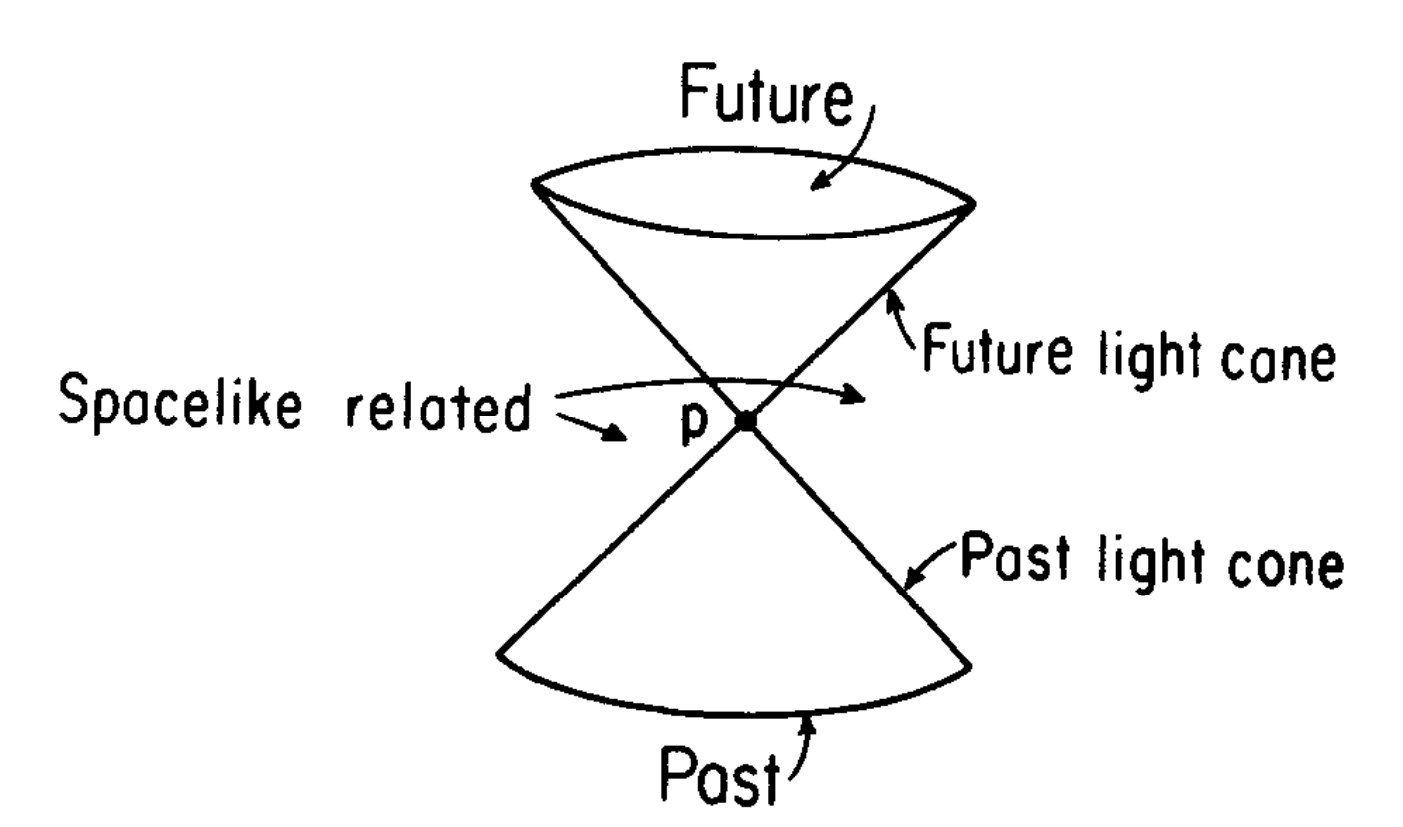
\includegraphics[scale=0.15]{lightcone.png}
\end{center}
\caption{Lightcone that shows that causal structure of spacetime in special relativity, the horizontal axes characterize spatial axes, and the vertical axis characterizes the time axis. Events that lie on the cone boundary cannot be reached by a material particle starting at $p$ but can be reached by a light signal emitted from $p$. The upper cone forms the future lightcone of $p$, and the lower cone forms the past lightcone of $p$.}
\end{figure}



\remark One might guess that the $\R^4$ Euclidean space is a suitable model for spacetime, but right now we do not know any \textit{global} property of spacetime, thus we shall not assume that spacetime has all the Euclidean structures.\\ 

In special relativity, neither the time interval nor the space interval between relatively simultaneous events, that are events determined to be simultaneous by a particular observer, has absolute significance. The quantity which is observer independent is the \textit{spacetime interval}, $I$, defined by
\begin{align}
I = -(\Delta t)^2 + \frac{1}{c^2}\left( (\Delta x)^2 +(\Delta y)^2 +(\Delta z)^2 \right)
\end{align}
where $\Delta t$ is the time interval, and $\Delta x,\, \Delta y,\, \Delta z$ describe the space interval. The spacetime interval $I$ and functions of $I$ are the only observer independent quantities characterizing the spacetime relationships between events. We shall later refer to $I$ as the metric of spacetime in in analogy to an ordinary Euclidean metric. \\


Spacetime should be a $4$-dimensional object as mentioned above, and intuitively, spacetime should locally look like Euclidean space, thus mathematically we would like to model spacetime by a $4$-dimensional manifold. In this text, an $n$-dimensional manifold $M$ is equipped with a set of charts $\psi:O_\alpha \to U_\alpha$, where $O_\alpha$ is an open subset of $M$ and $U_\alpha$ is an open subset of $\R^n$, precisely given by the following definition:
\begin{defn}
An $n$-dimensional real manifold $M$ of $C^\infty$ type is a set equipped with a collection of subsets $\mathcal{O} = \{O_\alpha \subseteq M |\, \alpha\in \mathcal{J}\}$ satisfying the following properties:\footnote{If not specified otherwise, $\mathcal{J}$ in this text denotes an index set.}
\begin{enumerate}[topsep=3pt,itemsep=-1ex,partopsep=1ex,parsep=1ex]
\item For all $p \in M$, there exists at least one $O_\alpha \in \mathcal{O}$ such that $p \in O_\alpha$. 
\item For $\alpha \in \mathcal{J}$, there exists a bijection $\psi_\alpha:O_\alpha \to U_\alpha$ where $U_\alpha\subseteq \R_n$ is open. 
\item If $O_\alpha, O_\beta\in \mathcal{O}$ overlap, then the map $\psi_\beta \circ \psi_\alpha^{-1}:\psi_{\alpha}(O_\alpha \cap O_\beta) \to \psi_{\beta}(O_\alpha \cap O_\beta)$ is of $C^\infty$ type, and the sets $\psi_{\alpha}(O_\alpha \cap O_\beta),\ \psi_{\beta}(O_\alpha \cap O_\beta)$ are open in $\R^n$. 
\end{enumerate}
Here the set $\mathcal{O}$ is called the cover of $M$. The cover $\mathcal{O}$ and the chart family $\{\psi_\alpha \mid \alpha \in \mathcal{J}\}$ are assumed to be maximal.
\end{defn}
 
The manifolds are further considered to be Hausdorff and paracompact. In a sense similar to what we have done in Math 635, the set $V_p$ of tangent vectors at a point $p \in M$ can be defined using the one-to-one correspondence between vectors and directional derivatives of the inverse of the charts $\phi$.\\

\subsection{Vector Spaces on Manifolds}
The tangent vectors on the manifold are viewed as the \textit{infinitesimal displacements} about a point on the manifold. In many situations, one is given a manifold without an embedding of it in $\R^n$, thus it is important to define a tangent vector in a way that refers only to the intrinsic structure of the manifold, not to its possible embeddings in $\R^n$. A vector $v=(v^1, v^2, \cdots, v^n) \in \R^n$ defines the directional derivative operator $\sum_\mu v^\mu(\pd/ \pd x^\mu)$ and vice versa. Directional derivatives are characterized by the linearity and Leibnitz rule behavior when acting on functions.
\begin{defn}
Let $M$ be an $n$-dimensional real manifold, and let $\mathcal{F}$ denote the collection of $C^\infty$  functions from $M$ to $\R$. We define a tangent vector $v$ at $p \in M$ to be a function $v:\mathcal{F}\to \R$ which is linear and obeys the Leibnitz rule, as characterized by
\begin{enumerate}[topsep=3pt,itemsep=-1ex,partopsep=1ex,parsep=1ex]
\item $v(af+bg) = av(f) + bv(g) $ for $f,g \in \mathcal{F}$ and $a,b \in \R$,
\item $v(fg) = f(p) v(g) + g(p) v(f)$ for $f,g \in \mathcal{F}$.
\end{enumerate}
\end{defn}

\note From Definition 1.0.2, we see immediately that if $h \in \mathcal{F}$ is a constant function denoted by $h(q) = c$ for any $q \in M$, then $v(h) = 0$ for any tangent vector $v$. As we have $v(h\cdot h) = 2cv(h)$ whereas $v(h\cdot h) = v(ch) = cv(h)$. \\

\begin{thm}[Theorem 2.2.1 on \txt]
Let $M$ be an $n$-dimensional manifold, and let $p \in M$, $V_p\coloneqq T_pM$ denote the tangent space at $p$, then $T_pM$ has dimension $n$.
\end{thm}
\begin{proof}[Proof sketch.]
Let $\mathcal{F}$ denote the collection of $C^\infty$  functions from $M$ to $\R$. The key of the proof is to show that the function $e_\mu: \mathcal{F}\to \R$ defined by the following defines a basis vector for the vector space $V_p$:
\begin{align*}
e_\mu(f) = \left.\frac{\pd}{\pd x^\mu}(f \circ  \psi^{-1})\right|_{\psi(p)}
\end{align*}
where $\psi$ is a chart that contains $p$ in its domain of definition, and $f \in \mathcal{F}$. If one uses a different chart $\psi'$, we would obtain a different coordinate basis $\{e'_\mu \mid \mu \in \N_n\}$ with similar definition, using the chain rule, we can write the following:
\begin{align*}
e_\mu = \sum_{\nu=1}^n \left.\frac{\pd (x')^\nu}{\pd x^\mu}\right|_{\psi(p)}e_\mu'
\end{align*}
where $(x')^\nu$ denotes the $\nu$-th component of the map $\psi'\circ \psi^{-1}$. Hence the components $(v')^\nu$ of a vector $v$ in the coordinate basis $\{e_\mu'\mid \mu\in \N_n\}$ are related to the components $v^\mu$ in the coordinate basis $\{e_\mu\mid \mu\in \N_n\}$ by the vector transformation law:
\begin{align}
(v')^\nu = \sum_{\mu}^n v^\mu \frac{\pd (x')^\nu }{\pd x^\mu}
\end{align}
\end{proof}

\remark The basis $\{e_\mu\mid \mu \in \N_n\}$ of $V_p$ introduced in Theorem 1.1 is called a \textit{coordinate basis} and is the natural basis equipped on $V_p$. \footnote{For notations on \txt, $e_\mu$ is denoted as $X_\mu$, or more generally, $\pd/\pd x^\mu$. }\\

\begin{defn}
A smooth curve on a manifold $M$ is a $C^\infty$ function $c:U \to M$, where $U$ is a connected subset of $\R$. For $f \in C^\infty(M, \R)$, let $T(f)$ be the derivative of $f\circ c:\R \to \R$, that is $T(f) = (d/dt)(f\circ c)$, here $T(f)$ is called the tangent vector field of $c$, and at each $p \in M$, $T(f)|_p$ is called the tangent vector of $c$ at $p$.
\end{defn}


\note From Definition 1.1.1, for $f \in C^\infty(M, \R)$, we can write:
\begin{align*}
T(f) = \frac{d}{dt}(f\circ c) = \sum_{\mu}\frac{\pd}{\pd x^\mu}(f\circ \psi^{-1}) \frac{dx^\mu}{dt} = \sum_\mu \frac{dx^\mu}{dt}e_\mu(f)
\end{align*}
where $e_\mu$ is defined similarly as in Theorem 1.1. Thus in any coordinate basis, the components of $T$ is given by $dx^\mu / dt$.\\

\begin{defn}
A vector field $V$ on a manifold $M$ is a function which associates each point $p \in M$ a vector $v \in T_pM$. A vector field $v$ is smooth provided that $v(f)$ is smooth for all $f \in C^\infty(M, \R)$. The commutator $[v,w]$ of two smooth vector fields $V, W$ on $M$ is a vector field defined by $[V,W](f) = V(W(f)) - W(V(f))$. 
\end{defn}



\subsection{Tensors on Manifolds}
Given the notion of tangent vectors, the use of tensors arises when one wants to compute other quantities. It turns out that many quantities have a linear dependence on displacements. 

\begin{defn}
Given a tangent space $V= V_p$ of a manifold $M$ at point $p \in M$, a tensor $T$ of type $(k,l)$ over $V$ is a multilinear map of the form given by
\begin{align*}
T:\underbrace{V^*\times V^* \times \cdots V^*}_{k\text{ times}} \times \underbrace{V \times V \times \cdots \times V}_{l \text{ times}} \to \R
\end{align*}
An assignment of tensor over $V_p$ for each $p \in M$ is called a tensor field on $M$. The collection of $(k,l)$ tensor is a $n^{(k+l)}$-dimensional vector space denoted as $\mathcal{T}(k,l)$. 
\footnote{Here and thereafter $V^*$ denotes the dual space of the vector space $V$. $V^{**}$ denotes the dual space of $V^*$, and is equipped with the canonical isomorphism $M:V \to V^{**}$ which sends $v\in V$ to a map in $V^{**}$ whose value on $w^* \in V^*$ reads $w^*(v)$.}
\end{defn}

\remark As such, a $(0,1)$ tensor over a vector field $V$ is a dual vector in $V^*$, and a $(1,0)$ tensor over $V$ is a dual of dual vector in $V^{**}$.\\

\begin{defn}
The contraction of a $(k,l)$ tensor with respect to its $i$-th dual-vector and $j$-th vector components is a map $C:\mathcal{T}(k,l) \to \mathcal{T}(k-1,l-1)$ defined by:
\begin{align*}
CT = \sum_{\sigma=1}^n T(\cdots, v^{\sigma^*}, \cdots, v_{\sigma},\cdots) 
\end{align*}
where $\{v_\sigma \mid \sigma \in \N_n\}$ and $\{v^{\sigma^*}\mid \sigma \in \N_n\}$ are the basis of $V$ and $V^*$, respectively, and the $v^{\sigma^*}$ and $v_\sigma$ are inserted into the $i$-th dual-vector and $j$-th vector component of $T$. 
\end{defn} 

\begin{defn}
The outer product of a $(k,l)$ tensor $T$ and a $(k',l')$ tensor $T'$ over a vector space $V$ is a $(k+k', l+l')$ tensor denoted as $T \otimes T'$ defined by:
\begin{align*}
(T&\otimes T')(v^{1^*}, v^{2^*} \cdots, v^{k^*}, v^{(k+1)^*}, \cdots, v^{(k+k')^*}, w_{1}, w_{2} \cdots, w_{l}, w_{l+1}, \cdots, w_{l+l'})\\
&= T(v^{1^*}, v^{2^*} \cdots, v^{k^*},w_{1}, w_{2} \cdots, w_{l} )\cdot T'(v^{(k+1)^*},\cdots, v^{(k+k')^*},w_{l+1}, \cdots, w_{l+l'} )
\end{align*}
where $v^{n^*}$ are dual vectors in $V^*$ and $w_n$ are vectors in $V$. 
\end{defn}

\begin{lem}
Every tensor $T$ of type $(k,l)$ over an $n$-dimensional vector space $V$ can be expressed as a sum of simple tensors:
\begin{align*}
T = \sum_{\substack{\mu_1 ,\,\mu_2,\,\cdots \mu_k,\, \in \N_n\\ \nu_1,\, \nu_2,\,\cdots,\,\nu_l \in \N_n}}(T^{\mu_1 \mu_2\cdots \mu_k}{}_{\nu_1\nu_2\cdots\nu_l})v_{\mu_1}\otimes v_{\mu_2}\otimes \cdots \otimes v_{\mu_k}\otimes v^{\nu_1^*}\otimes v^{\nu_2^*}\otimes \cdots \otimes v^{\nu_l^*}
\end{align*}
where $\{v_{\mu_i}\mid \mu_i \in \N_n\}$ is a basis of $V$ and $\{v^{\nu_i^*}\mid \nu_i \in \N_n\}$ is the corresponding dual basis of $V^*$, $T^{\mu_1 \mu_2\cdots \mu_k}{}_{\nu_1\nu_2\cdots\nu_l}\in \R$ is called the components of the tensor $T$ with respect to the given basis of $V$. Here we have taken the convention that, $v_{\mu_i}$ and $v^{\nu_i^*}$ satisfy the followings:
\begin{align*}
v^{\mu_j^*}v_{\mu_i} = \delta^{\mu_j}{}_{\mu_i} \qquad\quad\text{and}\quad\qquad v^{\nu_i^*}v_{\nu_j} =\delta^{\nu_i}{}_{\nu_j}
\end{align*}
The contraction of $T$ with respect to its $i$-th dual-vector and $j$-th vector components as in Definition 1.1.4 then has components given by:
\begin{align*}
(CT)^{\mu_1  \mu_2 \cdots  \mu_{k-1}}{}_{\nu_1\nu_2\cdots\nu_{l-1}} = \sum_{\sigma=1}^n T^{\mu_1  \mu_2\cdots\sigma \cdots \mu_k}{}_{\nu_1\nu_2\cdots\sigma\cdots\nu_l}
\end{align*}
with $\sigma$ being inserted into the $i$-th dual-vector and $j$-th vector components. The tensor product of a $(k,l)$ tensor $T$ and a $(k', l')$ tensor $T'$ has components given by:
\begin{align*}
(T\otimes T')^{\mu_1 \mu_2\cdots \mu_{k+k'}}{}_{\nu_1\nu_2\cdots\nu_{l+l'}} = T^{\mu_1 \mu_2\cdots \mu_{k}}{}_{\nu_1\nu_2\cdots\nu_{l}}  \cdot (T')^{\mu_{k+1}\cdots \mu_{k-k'}}{}_{\nu_{l+1}\cdots\nu_{l-l'}} 
\end{align*}
\end{lem} 


For notations, given an $n$-dimensional vector space $V$ with it basis $\{\pd/\pd x^i \mid i\in \N_n\}$, the associated dual basis of $V^*$ is denoted as $\{dx^i \mid i \in \N\}$. \\

\note Let $V$ be an $n$-dimensional vector space with its basis $\{v_\nu \mid \nu \in \N_n\}$, using Eq. (1.2), via the Inverse Function Theorem, and by requiring the basis vectors $v^{\mu^*}$ for $V^*$ to satisfy $v^{\mu^*}v_\nu = \delta^\mu{}_\nu$, we obtain the \textit{dual vector transformation law} for the components $w_\mu$ of a vector $w$:
\begin{align}
w_{\mu'}' = \sum_{\mu=1}^n w_\mu \frac{\pd x^\mu}{\pd (x')^{\mu'}}
\end{align}
where $x^\nu$ denotes the $\nu$-th component of the chart transition function $\psi\circ (\psi')^{-1}$. Combining one obtains the \textit{tensor transformation law} for components of a $(k,l)$ tensor $T$:
\begin{align}
(T')^{\mu_1 \cdots  \mu_{k}}{}_{\nu_1 \cdots \nu_{l}}  = \sum_{\mu_i,\, \nu_i \in \N_n}(T^{\mu_1 \cdots  \mu_{k}}{}_{\nu_1 \cdots \nu_{l}} )\frac{\pd (x')^{\mu_1'}}{\pd x^{\mu_1}}\cdots\frac{\pd (x')^{\mu_k'}}{\pd x^{\mu_k}}\frac{\pd x^{\nu_1}}{\pd x^{\nu_1'}}\cdots \frac{\pd x^{\nu_l}}{\pd x^{\nu_l'}}
\end{align}
\note In the rest of the text, a tensor $T$ of type $(k,l)$ is denoted as $T^{a_1a_2\cdots a_k}{}_{b_1b_2\cdots b_l}$ or simply $T^{a_1\cdots a_k}{}_{b_1\cdots b_l}$, with lower-case-letters subscripts and superscripts. The components of $T$ are denoted using greek-letters subscripts and superscripts $T^{\alpha_1\alpha_2\cdots \alpha_k}{}_{\beta_1\beta_2\cdots \beta_l}$. Vectors $v$ in the domain of definition of $T$ are denoted using superscripts $v^{b_i}$ such that $T^{a_1\cdots a_k}{}_{b_1\cdots b_i \cdots b_l}v^{b_i}$ is a $(k, l-1)$ tensor, that is the $i$-th vector component of $T$ is evaluated at $v^{b_i}$. A dual vector $w$, on the other hand, has vector space as a natural domain of definition, hence is viewed as a $(0,1)$ tensor, denoted using subscripts $w_{a_i}$. 

\subsection{The Metric Tensor}
\begin{defn}
In the theory of general relativity, a metric $g$ on a manifold $M$ is a symmetric non-degenerate tensor field of type $(0,2)$ defined on $M$. Components of $g$ are usually denoted as $g_{\mu\nu}$, and $g$ has the form:
\begin{align*}
g = \sum_{\mu, \nu} g_{\mu\nu}dx^\mu \otimes dx^\nu
\end{align*}
Conventionally, one might employ the compact notation for $g$:
\begin{align*}
ds^2 = \sum_{\mu,\nu}g_{\mu\nu}dx^\mu dx^\nu
\end{align*}
where the tensor outer product $\otimes$ notation is omitted.
\end{defn}

\remark The metric can be viewed as an inner product on the tangent space at each point in $M$. However, from Definition 1.1.6,  a metric tensor in the theory of general relativity is not necessarily positive definite.\\

\begin{thm}
Given a metric $g$ on a manifold $M$, one can find an orthonormal basis $\{v_1,v_2,\cdots, v_n\}$ of the tangent space at each $p$ in the spacetime manifold $M$, that is a basis that makes $g(v_i,v_j) = 0$ if $i\neq j$ and $g(v_i,v_j) = \pm 1$ for $i=j$. It is not hard to check that the number of basis vectors $v_i$ corresponding to $g(v_i,v_i) = +1$ and the number with $g(v_i,v_i) = -1$ are independent of the choice of such orthonormal basis. The number of the $+$ and $-$ signs occuring is called the \textit{signiture} of the metric. The metric equipped on a spacetime manifold $M$ usually has a signiture $(-,+,+,+)$, as in the next few examples. 
\end{thm}



\remark A positive definite metric, that is a metric with all-plus signature is called a Riemannian metric. A metric with a signature like those on spacetime, one minus and the remainder plus, is called a Lorentzian metric.

\begin{defn}
A manifold equipped with a Lorentzian metric is called a Lorentzian manifold.  
\end{defn}

\example Probably the simplest example of a Lorentzian manifold is the flat spacetime equipped with the Minkowski metric
\begin{align}
ds^2 = -c^2dt^2 + dx^2 + dy^2 + dz^2 = \eta_{\mu\nu} dx^{\mu}dx^\nu\,.
\end{align}
where $(t,x,y,z)$ is a coordinate in the spacetime manifold $M$. \\
In matrix form, the Minkowski metric can be represented by 
\begin{align*}
\eta = \bmat{-c^2 & 0 & 0 & 0\\
0 & 1 & 0 & 0\\
0 & 0 & 1 & 0\\
0 & 0 & 0 & 1}\, .
\end{align*}
Here $c$ is a constant, which is interpreted as the speed of light. The flat spacetime is in fact used more often in the theory of special relativity. In special relativity, an event is defined as a single moment in space and time, characterized uniquely by a coordinate $(t,x,y,z)$. One can then introduce the spacetime interval between two events,
\begin{align*}
I = -(c\Delta t)^2 + (\Delta x)^2 + (\Delta y)^2 + (\Delta z)^2 = \eta(z_1-z_2) = \eta_{\mu\nu}\Delta x^{\mu}\Delta x^{\nu}\, ,
\end{align*}
which is a quantity that is invariant for all observers in any inertial frames. \footnote{More details about special relativity in a context without differentiable geometry can be found in Jinyan's notes for the class Physics 360 - Honors Physics, taught by Henriette Elvang at the University of Michigan in Fall 2021.}\\

\example Another example of a Lorentzian manifold is a spacetime equipped with the Schwarzschild metric given by
\begin{align}
ds^2 = -\left( 1 - \frac{2Gm}{rc^2}\right)\, c^2 \, dt^2 + \left( 1 - \frac{2Gm}{rc^2}\right)^{-1} \, dr^2 + r^2 d\Omega^2\, ,
\end{align}
where $d\Omega^2 = d\theta^2+\sin^2(\theta) \,d\phi^2 $ is the standard metric on the $2$-sphere, $G$ is the gravitation constant, $m$ is a constant with the dimensions of mass. Note that, except at the origin, the Schwarzschild metric approaches the spherical form of the Minkowski metric as $m$ approaches $0$, or as $r$ approaches infinity. Note here (1.6) is an exact solution to Einstein's field equations that describes the gravitational field outside a spherical mass, which we shall discuss in next Chapter. Eq. (1.6) is helpful for describing slowly rotating astronomical objects, especially the curved spacetime around a black hole singularity. 

\newpage
\section[Derivative Operators on a Manifold]{\color{red} Derivative Operators on a Manifold\color{black}}
\begin{defn}
A derivative operator, or the covariant derivative operator, on a manifold $M$ is an operator $\nabla_a$ that associates any $(k, l)$ tensor with a $(k, l+1)$ tensor, and $\nabla_a$ itself satisfies the following properties:
\begin{enumerate}
\item Linearity. For $A,B \in \mathcal{T}(k, l)$, and $\alpha,\beta \in \R$, we have: 
$$\nabla_a(\alpha A^{c_1 \cdots  c_k}{}_{b_1 \cdots b_l} + \beta B^{c_1\cdots  c_k}{}_{b_1 \cdots b_l}) = \alpha \nabla_a A^{c_1 \cdots  c_k}{}_{b_1 \cdots b_l} + \beta \nabla_a B^{c_1 \cdots  c_k}{}_{b_1 \cdots b_l}$$
\item Sanctification of the Leibnitz Rule. For $A\in \mathcal{T}(k, l)$ and $B\in \mathcal{T}(k',l')$, we have: 
\begin{align*}
\nabla_a&\left(A^{c_1 \cdots  c_k}{}_{b_1 \cdots b_l} B^{d_1 \cdots  d_k'}{}_{e_1 \cdots e_l'}  \right)\\
&=\left( \nabla_a  A^{c_1 \cdots  c_k}{}_{b_1 \cdots b_l} \right)B^{d_1 \cdots  d_k'}{}_{e_1 \cdots e_l'}  + A^{c_1 \cdots  c_k}{}_{b_1 \cdots b_l} \left( \nabla_a B^{d_1 \cdots  d_k'}{}_{e_1 \cdots e_l'} \right)
\end{align*}
\item Commutativity with contraction. For all $A \in \mathcal{T}(k,l)$, we have:
\begin{align*}
\nabla_a (A^{c_1  c_2 \cdots  d  \cdots  c_k}{}_{b_1 b_2 \cdots  d  \cdots  b_l}) = \nabla_a A^{c_1  c_2 \cdots  d  \cdots  c_k}{}_{b_1 b_2 \cdots  d  \cdots  b_l}
\end{align*}
\item Consistency with the notion of tangent vectors as directional derivatives. For all $f \in C^\infty(M, \R)$ and $t=t^a \in V_p$ for some $p \in M$, we have:
\begin{align*}
t(f) = t^a\nabla_a f
\end{align*}
\item Torsion free. For all $f \in C^\infty (M, \R)$, we have:
\begin{align*}
\nabla_a\nabla_b f = \nabla_b \nabla_a f
\end{align*}
\end{enumerate}
\end{defn}
\remark As in Definition 2.0.1, even though we denote a derivative operator on a manifold $M$ as $\nabla_a$, the operator $\nabla_a$ itself is not a tensor, nor a dual vector. \\

\note It is not hard to verify that such a derivative operator $\nabla_a$ defined on a manifold $M$ exists. Given a chart $\psi$ on $M$, in the region $U \subseteq M$ covered by $\psi$ we can define a derivative operator $\pd_a$, called the ordinary derivative, by letting the tensor $\pd_a T^{b_1 \cdots b_k}{}_{c_1 \cdots  c_l} $ have components given by $\pd(T^{\mu_1 \cdots \mu_k}{}_{\nu_1 \cdots  \nu_l})/\pd x^\sigma$ in the given coordinate basis. Note further that the ordinary derivative operator is coordinate dependent. 

\begin{lem}
Let $\nabla_a$ and $\that{\nabla}_a$ be derivative operators on a manifold $M$, for $T \in \mathcal{T}(k,l)$, we have:
\begin{align*}
\nabla_a &T^{b_1 \cdots  b_k}{}_{c_1 \cdots c_l} \\
&= \that{\nabla}_a T^{b_1 \cdots  b_k}{}_{c_1 \cdots c_l} +\sum_i C^{b_i}{}_{ad}T^{b_1 \cdots  d \cdots  b_k}_{}{c_1 \cdots  c_l}-\sum_j  C^{d}{}_{ac_j}T^{b_1 \cdots   b_k}{}_{c_1 \cdots  d \cdots  c_l} \tag{1.8}
\end{align*}
where $C^{a}{}_{bc}$ is an $(1,2)$ tensor field on $M$. Note here the $i$-th dual-vector component of $T^{b_1 \cdots  d \cdots  b_k}{}_{c_1 \cdots  c_l}$ is labeled as $d$ instead of $b_i$, and the $j$-th component of $T^{b_1 \cdots   b_k}{}_{c_1 \cdots  d \cdots  c_l}$ is labeled as $d$ instead of $c_j$. 
\end{lem} 

Lemma 2.0.1 suggests a relation between two derivative operators on a manifold $M$. For a vector field $t^a$ on $M$, Eq. (1.8) reduces to the following:
\setcounter{equation}{8}
\begin{align}
\nabla_at^b = \that{\nabla}_at^b +C^b{}_{ac} t^c
\end{align}
where $C^b{}_{ac}$ is a (1,2) tensor field on $M$. In particular, in the case where $\that{\nabla}_a$ in Eq. (1.9) is taken to be the ordinary derivative operator $\pd_a$ associated to a given chart, the tensor field $C^{b}{}_{ac}$ is denoted as $\Gamma^b{}_{ac}$ instead, and $\Gamma^b{}_{ac}$ is called the Christoffel symbol, satisfying the following:
\begin{align}
\nabla_at^b = \pd_at^b +\Gamma^b{}_{ac} t^c
\end{align}

\begin{lem}
Let $\nabla_a$ be a derivative operator on a manifold $M$, let $v^a$ and $w^b$ be vector fields on $M$, then we have $[v,w]^b\coloneqq [v,b]$ being a vector field on $M$ satisfying the following:
$$[v,w]^b = v^a \nabla_a w^b - w^a \nabla_a v^b$$
\end{lem}

\begin{defn}
Given a derivative operator $\nabla_a$ on a manifold $M$ and a curve $c: I \to M$ on $M$, where $I$ is a connected subset of $\R$, a vector $v^a$ given at each point $p$ on the curve $c$ is said to be parallelly transported along $c$ whose tangent is $t^a$ provided that we have $t^a \nabla_a v^b=0$ holds along the curve. A tensor $T^{b_1 \cdots  b_k}{}_{c_1 \cdots  c_k}$ is said to be parallelly transported along $c$ provided that we have $t^a \nabla_aT^{b_1 \cdots  b_k}{}_{c_1 \cdots  c_k}$ holds along the curve. 
\end{defn}

\note By specifying a coordinate system, $t^a \nabla_a v^b=0$ as in Definition 2.0.2 has a form:
\begin{align*}
t^a \pd_a v^b + t^a \Gamma^b{}_{ac}v^c = 0
\end{align*}
in terms of components, we have:
\begin{align*}
\frac{dv^\nu}{dt} + \sum_{\mu, \lambda} t^\mu \Gamma^{\nu}{}_{\mu\lambda}v^\lambda = 0
\end{align*}
\hfill\break
\hfill\break
The definition of parallel transport allows us to \textit{connect} tangent vector spaces at different points on a manifold, hence the derivative operator $\nabla_a$ is sometimes called the \textit{connection} on the manifold. Practically, one would like to have a derivative operator that is compatible with the metric defined on a manifold $M$. That is, when vectors $v^b$ and $w^c$ are parallelly transported along curves on the manifold, $g_{bc}v^bw^c$ should be invariant, that is $t^a\nabla_a (g_{bc}v^bw^c) = 0$, which leads to $\nabla_a g_{bc} = 0$. 

\begin{thm}[Theorem 3.1.1 on \txt]
Let $g_{bc}$ be a metric on a manifold $M$, there exists a unique derivative operator $\nabla_a$ on $M$ that is compatible with $g_{ab}$, that is $\nabla_a g_{bc} = 0$ everywhere on $M$. In which case the tensor field $C$ in Eq. (1.8) satisfies the following for any given $\that{\nabla}_a$:\footnote{A torsion free derivative operator $\nabla_a$ that is compatible with the given metric on the manifold is called the Levi-Civita Connection on $M$.}
\begin{align}
C^c{}_{ab} = \frac{1}{2}g^{cd}\left(\that{\nabla}_ag_{bd} + \that{\nabla}_b g_{ad} - \that{\nabla}_dg_{ad} \right)
\end{align}
\end{thm}
\newpage
\begin{cor}
From Theorem 2.1, in terms of a given ordinary derivative operator, the Christoffel symbol in Eq. (1.10) that makes $\nabla_a$ being compatible with the metric on $M$ has the following form:
\begin{align*}
\Gamma^c{}_{ab} = \frac{1}{2}g^{cd}\left( \pd_a g_{bd}+\pd_b g_{ad} - \pd_d g_{ab}\right)
\end{align*}
The components of the Christoffel symbol is given by the following:
\begin{align*}
\Gamma^\sigma{}_{\mu \nu} = \frac{1}{2}\sum_\sigma g^{\rho \sigma}\left( \frac{\pd g_{\nu \sigma}}{\pd x^\mu} + \frac{\pd g_{\mu \sigma}}{\pd x^\nu} - \frac{\pd g_{\mu\nu}}{\pd x^\sigma}\right)
\end{align*}
\end{cor}
\newpage

\section[Curvature and Geodesics of a Manifold]{\color{red}Curvatures and Geodesics\color{black}}
Let $M$ be a manifold and let $p,q \in M$, with tangent spaces $V_p$ and $V_q$. In general, parallelly transporting a vector from $V_p$ to $V_q$ depends on the path connecting $p$ and $q$. We can use the path dependence of parallel transport to define an intrinsic notion of curvature. \\

Let $\nabla_a$ be a derivative operator on a manifold $M$, and let $w_c$ be a dual vector field on $M$, it is not hard to show that $\nabla_a \nabla_b w_c -\nabla_b\nabla_aw_c$ can be viewed as a $(1,3)$ tensor acting on $w_d$, such that the following (Eq. (3.2.3) on \txt) holds:
\begin{align*}
\nabla_a \nabla_b w_c -\nabla_b\nabla_aw_c = R_{abc}{}^d w_d
\end{align*}
where the operator $R_{abc}{}^d$ is called the Riemannian curvature tensor. One also finds that the action of $R_{abc}{}^d$ on a vector field $t^c$ gives the following:
\begin{align*}
\nabla_a\nabla_b t^c - \nabla_b\nabla_a t^c = -R_{abd}{}^c t^d
\end{align*}
from which induction gives:
\begin{align*}
(\nabla_a\nabla_b - \nabla_b \nabla_a) T^{c_1 \cdots  c_k}{}_{d_1 \cdots  d_l} = -\sum_{i=1}^k R_{abe}{}^{c_i}T^{c_1 \cdots  e  \cdots  c_k}{}_{d_1\cdots d_l} + \sum_{j=1}^l R_{abd_j}{}^e T^{c_1\cdots c_k}{}_{d_1\cdots e\cdots d_l}
\end{align*}
\begin{lem}
The Riemannian curvature tensor $R_{abc}{}^d$ on a manifold satisfies the followings:  \footnote{$R_{[abc]}{}^d = (R_{abc}{}^d + R_{bca}{}^d + R_{cab}{}^d - R_{bac}{}^d - R_{acb}{}^d - R_{cba}{}^d)/6$}\,\footnote{$\nabla_{[a}R_{bc]d}{}^e = (\nabla_aR_{bcd}{}^e+\nabla_bR_{cad}{}^e + \nabla_c R_{abd}{}^e - \nabla_bR_{acd}{}^e - \nabla_aR_{cbd}{}^e - \nabla_cR_{bad}{}^e)/6$}
\begin{enumerate}[topsep=3pt,itemsep=-1ex,partopsep=1ex,parsep=1ex]
\item $R_{abc}{}^d = -R_{bac}{}^{d}$
\item $R_{[abc]}{}^d = 0$    
\item $R_{abcd} = -R_{abdc}$ for the $\nabla_a$ that satisfies $\nabla_ag_{bc}=0$
\item The Bianchi identity holds, that is $\nabla_{[a}R{}_{bc]d}{}^e = 0$
\end{enumerate}
\end{lem}

From Lemma 3.0.1, we see here the trace of $R_{abc}{}^d$ over its first two or last two indices vanishes, while its trace over the second and fourth, or the first and third, indices defines the Ricci curvature tensor $R_{ac}$, given by:
\begin{align*}
R_{ac} \coloneqq R_{abc}{}^b
\end{align*}
where we have an obvious property $R_{ac} = R_{ca}$. The scalar curvature $R$ is defined by the following:
\begin{align*}
R\coloneqq R_a{}^{a}
\end{align*}
Bianchi identity leads to an important equation satisfied by $R_{ab}$, that is we have:
\begin{align}
\nabla_a R_{bcd}{}^a + \nabla_b R_{cd} - \nabla_c R_{bd} = 0
\end{align}
Defining the tensor $G_{ab}$ by the following:
\begin{align*}
G_{ab}\coloneqq R_{ab} - \frac{1}{2}R\cdot g_{ab}
\end{align*}
we obtain the following from (1.12):
\begin{align*}
\nabla_a R_c{}^a + \nabla_b R_c{}^d - \nabla_c R = 0\qquad\Rightarrow \qquad  \nabla^a G_{ab} = 0
\end{align*}
where the tensor $G_{ab}$ is called the Einstein tensor. \\

\begin{defn}
Let $\nabla_a$ be a derivative operator on a manifold $M$, a geodesic on $M$ is a curve $c:I \to M$, where $I$ is a connected subset of $\R$, whose tangent vector $t^a$ satisfies $t^a\nabla_a t^b = 0$ along $c$. 
\end{defn}

Given a derivative operator $\nabla_a$ on a manifold $M$, one can in fact reparametrize any curve whose tangent vector $t^a$ satisfies $t^a \nabla_a t^b = \alpha  t^b$ for some $\alpha \in C^\infty (M, \R)$ to obtain a geodesic on $M$. Hence we only consider curves which are affinely parametrized, that is $t^a\nabla_a t^b = 0$. Written in coordinate basis components, the geodesic equation $t^a \nabla_a t^b = 0$ reads the following:
\begin{align}
\frac{d^2 x^\mu}{dt^2} + \sum_{\sigma, \nu}\Gamma^{\mu}{}_{\sigma \nu} \frac{dx^\sigma}{dt}\frac{dx^\nu}{dt} = 0\, .
\end{align}
which is a coupled system of $n$ second order ODE for $n$functions $x^\mu$. Given initial value of $x^\mu$ and $dx^\mu/dt$, unique solution to (1.13) always exists by the Cauchy-Lipschitz Theorem. \\

\begin{thm}
Let $M$ be a manifold equipped with the Levi-Civita connection $\nabla_a$. Given $p\in M$ and and tangent vector $t^a \in V_p$, there exists a unique geodesic through $p$ with tangent vector $t^a$ at $p$. 
\end{thm}

\note From the notion of existence and uniqueness of geodesic at a given point and given velocity on the manifold, one can define the exponential map, normal coordinates, and polar coordinates locally on the manifold.\\ 

\note For computations of curvatures in coordinate components, one makes use of Section 3.4 - \textit{Methods for Computing Curvature} on \txt. 

\subsection{The Lengths of the Geodesics in Lorentzian Manifolds}
\begin{defn}
Denoting the tangent vector of a geodesic $c:I \to M$ on a Lorentzian manifold $M$ as $T^a$, $c$ is said to be \textit{timelike} provided that $g_{ab}T^aT^b<0$ everywhere, $c$ is said to be \textit{null} provided that $g_{ab}T^aT^b = 0$ everywhere, and $C$ is said to be \textit{spacelike} if $g_{ab}T^aT^b >0$ everywhere. The length $l$ of spacelike $c$ is defined by:
\begin{align}
l = \int_{t \in I}(g_{ab}T^aT^b)^{1/2}\, dt\, .
\end{align}
The length of the null geodesic is $0$. The \textit{proper time} of timelike $c$ is defined by:
\begin{align}
\tau = \int_{t \in I}(-g_{ab}T^aT^b)^{1/2}\, dt\, .
\end{align}
\end{defn}
Since the tangent vector of a geodesic is parallel transported, it has a constant norm, which ensures that geodesics in the Lorentzian manifold cannot change from timelike to spacelike or null.\\

\note Length of a curve is invariant under reparametrization. \\

\remark The geodesics in Riemannian manifolds are paths that extremize the length functional. A similar argument can be employed to show that the paths in Lorentzian manifolds extremize the length or the proper time. That is, curves that extremize proper time between two points are precisely the timelike geodesics, and the curves that extremize the length between two points are precisely the spacelike geodesic. In general relativity, \textit{gravity} is treated as a built-in feature of the spacetime structure, reflected by the metric $g_{ab}$. A test particle in spacetime is said to be \textit{free-falling} provided that the particle does not experience any non-gravitational force. As a result, timelike geodesics are the trajectories of massive free-falling test particles, and the proper time of the timelike geodesic is a quantity describing the time measured by a clock moving along the geodesic. Null geodesics are the trajectories of the massless free-falling test photons, and it has a proper time $0$. Two independent events in spacetime are spacelike related. \\

\begin{thm}
Given a Lorentzian manifold with its compatible derivative operator $\nabla_a$, the curves which extremize propertime between two points are precisely the timelike geodesics, and the curves which extremize length between two points are precisely the spacelike or null geodesics. 
\end{thm}
\note The proof of Theorem 3.2 is a direct application of variation calculation. \\

In Riemannian manifolds, one can find curves of arbitrarily long length connecting two points, while the length between two points are bounded below. In Lorentzian manifolds, in contrast, one can find timelike curves of arbitrarily small proper time connecting points. In some spacetime, the proper time of timelike curves connecting the two given points need not be bounded above, but if a curve of greatest proper time exists, it must be a timelike geodesic. \\


\subsection{Deviation of Geodesics}
Let $\mathcal{G} = \{\gamma_s\mid s \in \R\}$ denote a smooth one-parameter family of geodesics parametrized by the affine parameter $t$. Consider the map $F:U \to M \ \ \  (t,s) \mapsto \gamma_s(t)$ with $U \subseteq \R$, which is smooth, injective, and has a local smooth inverse. Let $Y$ denote the $2$-dimensional submanifold of $M$ spanned by the curves $\mathcal{G}$. Here $Y$ has natural coordinates $(s,t)$. The vector field $T^a\coloneqq (\pd /\pd t)^a$ is tangent to the family of geodesics, and hence we have $T^a \nabla_a T^b = 0$, whereas the vector field $X^a=(\pd /\pd s)^a$ represents the displacement to an infinitesimally nearby geodesics, and here $X^a$ is called the vector field of \textit{deviation vector}. Given the Levi-Civita connection $\nabla_a$ on the manifold of interest, by re-scaling parameter $t$ by an $s$-dependent factor, one can ensure that $g_{ab} T^a T^b$ does not vary with $s$. Here $X^a$ and $T^a$ are coordinate vector fields, hence they commute, and thus is not difficult to show that $X^aT_a$ is constant along each geodesic (pp. 43, 46 on \txt). Furthermore, by reparametrizing each $\gamma_s$ by adding a constant dependent on $s$ to the affine parameter $t$, we may ensure that the curve $C:\R \to M \ \ \ s\mapsto\gamma_s(0)$ is orthogonal to all the geodesics. Thus we have $X_aT^a = 0$ along $C$, and hence $X^aT_a = 0$ everywhere as $X^aT_a$ is constant along each geodesic. \\

With the constructions above, the quantity $v^a = T^b\nabla_b X^a$ gives the rate of change along a geodesic of the displacement to an infinitesimally nearby geodesic, so $v^a$ may be interpreted as the relative velocity of an infinitesimally nearby geodesic. Similarly, we may interpret $a^d = T^c \nabla_c v^d = T^c \nabla_c(T^b \nabla_b X^d)$ as the relative acceleration of an infinitesimally nearby geodesic in the family $\mathcal{G}$. Simply derivation (Eq. (3.3.18) on \txt) shows that we have the following:
\begin{align}
a^d = -R_{cbe}{}^dX^bT^cT^e
\end{align}
Eq. (1.16) is referred as the \textit{geodesic deviation equation}.\\

\note One has $a^d =0$ for all families of geodesics if and only if $R_{abc}{}^d = 0$. Thus some geodesics will accelerator toward or away from each other if and only if the Riemannian curvature tensor of the manifold does not vanish everywhere. 




\newpage
\chapter{The Theory of Relativity}
\setcounter{section}{3}
%\section[Einstein's  Equivalence Principle]{\color{red}Einstein's  Equivalence Principle\color{black}}
%\textit{By Einstein, Equivalence Principle states that the law of the equality of the inertial and gravitational mass is equivalent to the assertion that the acceleration imparted to a body by a gravitational field is independent of the nature of the body.}\\
%
%Before moving on to the discussion of Einstein's Equation, here we present another method of deriving the geodesic equation (1.13). This method, first proposed by Steven Weinberg in 1972, provides a physical interpretation of the geodesic equation, that is the geodesic equation can be derived directly from the equivalence principle.
%
%\begin{proof}
%Here we show the key steps of the derivation of the geodesic equation from the equivalence principle, the details can be found in Ref. \cite{W} (pp. 70). We first consider a free-falling particle that does not accelerate in the neighborhood of a point-event $p \in M$. By the principle of equivalence, we can choose a free-falling coordinate system $X^\mu$ such that we have
%\begin{align*}
%\frac{d^2 X^\mu}{dT^2} = 0\,,
%\end{align*}
%where we have denoted $T = X^0$. By expanding using the chain rule and differentiating with respect to time, we can obtain
%\begin{align}
%\frac{d^2 x^\lambda}{dT^2} = -\frac{dx^\nu}{dT} \frac{dx^\alpha}{dT}\left( \frac{\pd^2 X^\mu}{\pd x^\nu \pd x^\alpha} \frac{\pd x^\lambda}{\pd X^\mu}\right)\,.
%\end{align}
%Now we define an affine connection by the use of Christoffel symbols
%\begin{align*}
%\Gamma_{\nu \alpha}^{\lambda} = \frac{\pd^2 X^\mu}{\pd x^\nu \pd x^\alpha}\frac{\pd x^\lambda}{\pd X^\mu}\,.
%\end{align*}
%Hence (6) becomes
%\begin{align}
%\frac{d^2 x^\lambda}{dT^2} = -\Gamma_{\nu \alpha}^\lambda\frac{dx^\nu}{dT} \frac{dx^\alpha}{dT}\, .
%\end{align}
%A change of coordinate applying to (2.7) yields a form of geodesic equation
%\begin{align}
%\frac{d^2 x^\lambda}{dt^2} = -\Gamma_{\nu \alpha}^\lambda \frac{dx^\nu}{dt}\frac{dx^\alpha}{dt} + \Gamma_{\nu \alpha}^0 \frac{dx^\nu}{dt} \frac{dx^\alpha}{dt} \frac{dx^\lambda}{dt}\,.
%\end{align}
%This completes the result.
%\end{proof}
%Also in Ref. \cite{W} (pp. 102), Weinberg gives another way of deriving the geodesic equation using the principle of general covariance, which emphasizes the formulation of physical laws using only those physical quantities of which the observers in different frames of reference could unambiguously correlate.\\

\section[Prerelativity and Motivations]{\color{red}Prerelativity and Motivations\color{black}}
Before the theory of relativity, it is assumed that the space manifold $M$ has the Euclidean structure . Each neighborhood of a point $p \in M$ can be covered by a chart $\phi$ whose inverse $\phi^{-1}: U\to M$ can be viewed as a composition of rotation and translation of the subset $U$ of $\R^3$, the so-obtained coordinate system is called the Cartesian coordinate system. The metric equipped on $M$, written in the Cartesian coordinate system, has the following form:
\begin{align}
h_{ab} = \sum_{\mu,\nu}h_{\mu \nu}(dx^\mu)_a (dx^\nu)_b
\end{align}
with $h_{\mu\nu} =1$ when $\mu=\nu$, and $h_{\mu\nu}=0$ when $\mu\neq \nu$. Note that the definition of $h_{ab}$ is independent of the choice of Cartesian coordinate system used to cover a neighborhood in $M$. Furthermore, as each $h_{\mu\nu}$ is constant, it is observed that we have $\pd_a h_{bc} = 0$, and consequently $\Gamma_{bc}{}^a$ vanishes for the given Cartesian coordinate system. Thus, the curvature of $M$ vanishes, in which case $M$ equipped with $h_{ab}$ is said to be \textit{flat}. From the geodesic equations (1.13), we deduce that the geodesics on $M$ are the \textit{straight lines} in Cartesian coordinates, in other words, straight lines in $\R^3$. The distance between two points on $M$, in accordance with Eq. (1.14), has the simple form given by the following:
\begin{align*}
l = \left((\Delta x^1)^2+(\Delta x^2)^2+(\Delta x^3)^2\right)^{1/2}
\end{align*}
where $\Delta x^i = x^i_{\text{final}} - x^i_{\text{initial}}$ is the $i$-th component displacement in the Cartesian coordinate system. Thus, we can conclude that, in prerelativity physics, the space can be viewed as the manifold $\R^3$ equipped with a flat Riemannian metric. \\

Quantities of physical interest in space must eventually be reducible to numbers as all experiments in physics measure numbers. However, many quantities of interest, such as magnetic field or the stress tensor, require the additional specification of a basis of vectors in order to produce numbers. Thus a general class of quantities of interests are maps of vectors and dual vectors into numbers. Any analytic map can be Taylor-expanded as a sum of multilinear maps, hence tensor fields encompass an extremely wide class of quantities. Indeed, the notion of tensor fields appears to be great enough so that essentially all quantities which one considers in physics can be viewed as tensor fields, and the laws of physics governing these quantities can be expressed as tensor equations. \\

\subsection{Principles of Covariance}
The following ideas, principles of covariance, played important roles in motivating the formulation of the theory general relativity and special relativity. \\

\textbf{The Principle of General Covariance}\\
\textit{The metric of space is the only quantity pertaining to space that can appear in the laws of physics. The form of the laws of physics should be the same in all inertial and accelerating frames.}\\

More specifically, the principle of general covariance states that there are no preferred vector fields or preferred bases of vector fields pertaining only to the structure of space which appear in any law of physics. The implication of the principle of general covariance is that a Christoffel symbol cannot appear by itself in any law of physics, as it is equivalent to specifying an ordinary derivative which is an additional geometric quantity pertaining to the space and is not derivable from the metric. Furthermore, the Christoffel symbol cannot appear in the law of physics as it coordinate components do not transform according to tensor transformation under general coordinate transformation. \\

\textbf{The Principle of Special Covariance}\\
\textit{Any physically possible set of measurements obtained by a family $\mathcal{O}$ of observers stationed in space also is physically possible set of measurements for another family $\mathcal{O}'$ of observers obtained by acting on $\mathcal{O}$ with an isometry $\phi$.}\\

The principle of special covariance implies the existence of an action of the isometry group on the states of physical fields being measured. One can use this group action to derive, or at least motivate, the possible laws governing the physical fields. \\

Suppose an object of physical interest in described by a tensor field $T$. If general covariance holds, then the equations governing $T$ should involve only $T$, the metric of space $h_{ab}$, and the quantities determined by $h_{ab}$, such as its derivative operator. Furthermore, all quantities measurable by $\mathcal{O}$ should be expressible as scalars resulting from contracting $T$ and its derivatives with the basis vector fields associated with $\mathcal{O}$. Let $\phi$ be an isometry, if special covariance holds, the action of $\phi$ on $T$ with produce a tensor field $\phi^*T$ which will satisfy the equations for the physical field and will yield the same measurable quantities for $\mathcal{O}'$ as $T$ yields for $\mathcal{O}$. \\

\remark Special covariance of the laws of physics for tensor fields implies that if we pick a coordinate system and write out the coordinate component equations without explicitly incorporating the metric into the equation but rather substituting everywhere its coordinate components $h_{\mu\nu}$, then the form of the equations will be preserved under the coordinate transformations corresponding to the isometries, for the simple reason that the numerical values of the components $h_{\mu\nu}$ remain unchanged under these transformations.\\

Historically, the formulations of special and general covariance played a large role in discussions of relativity theory, and indeed, the name of special and general relativity derive from these formulations of special and general covariance. 



\newpage
\section[Special Relativity]{\color{red}Special Relativity\color{black}}
In the theory of special relativity, it is assumed that the spacetime has the manifold structure of $\R^4$. It is assumed that there exist preferred families of motion in spacetime, referred to as \textit{inertial} or \textit{nonaccelerating} motions. \\

The inertial observers is further assumed can set up a rigid grid of metersticks, synchronize clocks placed at the gridpoints, \footnote{By clock synchronization, the inertial observer makes sure two given clocks give the same reading when they receive a signal sent out in a symmetrical manner by an observer stationed halfway between the two.} and label each event in spacetime by the grid coordinates $(x^1, x^2, x^3)$ and the clock reading $t$ at an event. The map of spacetime into $\R^4$ is called a \textit{global inertial coordinate system}. Indeed, many different global inertial coordinate systems are possible, hence the coordinate components of events do not have intrinsic meaning. While the spacetime interval between two events $\bar{x}$ and $x$, as defined by Eq. (1.1), or in units where $c=1$ given by the following has the same value for all global inertial coordinate systems and thus can be viewed as representing an intrinsic property of spacetime:
\begin{align}
I = -(t - \bar{t})^2 + (x^1 - \bar{x}^1 )^2 + (x^2 - \bar{x}^2 )^2 + (x^3 - \bar{x}^3 )^2 
\end{align}
\begin{defn}
In special relativity, the metric of spacetime is defined by the following:
\begin{align*}
\eta_{ab} \coloneqq \sum_{\mu,\nu=0}^3 \eta_{\mu\nu}(dx^\mu)_a(dx^\nu)_b
\end{align*}
with $\eta_{\mu\nu} = \text{diag}(-1,1,1,1)$, where $x^\mu$ denotes any global inertial coordinate system. 
\end{defn}
From Definition 5.0.1, we observe that the ordinary derivative operator of the global inertial coordinates satisfies $\pd_a\eta_{bc}=0$, and thus is the Levi-Civita connection on the spacetime equipped with $\eta_{ab}$. The curvature of spacetime equipped with $\eta_{ab}$ thus vanishes everywhere. The geodesics in spacetime equipped with $\eta_{ab}$ are the straight lines when expressed in global inertial coordinates. In particular, the timelike geodesics are precisely the world lines of inertial observers in spacetime. 



























Similar to the way that Maxwell's equations relate the distribution of charges and currents in space to the electromagnetic field, Einstein's field equations (EFE) allow us to correlate the distribution of matter in spacetime to the geometry of spacetime. Once we obtain the geometry of spacetime, the geodesics equation (3) can be used to compute the paths of free-falling particles in spacetime. \\

The laws of physics in general relativity are governed by two principles: (1) the principle of general covariance, that is the laws of physics should be the same in all inertial and accelerating frames; (2) we require that all equations must reduce to the equations that hold in the theory of special relativity in the case where $g_{\mu\nu}$ is flat. As we have mentioned, we will model the spacetime as a manifold $M$ equipped with a Lorentzian metric $g_{\mu\nu}$. The derivation of the EFE is based on modifying the equations that hold in special relativity under a flat metric, the full derivation is given in Ref. \cite{Wald} (pp. 68-72), here we will just state the result,
%Here we will make use of some notions from the theory of special relativity with differential geometry: Particle motions are represented by a timelike curve under a given metric $g_{ab}$; perfect fluids are described in terms of a $4$-velovity $u^\alpha$, a density $\rho$, and pressure $P$; The electromagnetic field is represented by an antisymmetric tensor $F_{ab}$. \footnote{More details about the tensor representation of electromagnetic field can be found in Jinyan's notes for the class Math 396 -  Honors Analysis, taught by Professor David Barrett in Winter 2022.} \\
%We define the $4$-velocity $u^\alpha$ of a particle in spacetime to be the unit vector tangent to its worldline. A free particle hence satisfies the geodesic equation of motion
%\begin{align*}
%u^\alpha \nabla_\alpha u^b=0
%\end{align*} 
%where $\nabla_a$ is the Levi-Civita connection associated to $g_{ab}$. The momentum of the particle is defined by $p^\alpha  = mu^\alpha$, where $m$ is the rest mass of the particle. The energy of the particle as determined by an observer who is present at the event of the particle's worldline at which the energy is measured is $E = -p_av^a$, where $v^a$ is the $4$-velocity of the observer. 
\begin{align}
R_{\mu\nu}- \frac{1}{2}Rg_{\mu \nu} = \kappa T_{\mu\nu}\,,
\end{align}
where $g_{\mu\nu}$ is the Lorentzian metric tensor, $R_{\mu \nu}$ is the Ricci curvature tensor, $R$ is the scalar curvature, $\kappa$ is the Einstein gravitation constant, and $T_{\mu\nu}$ is the stress-energy-momentum tensor. Another cosmological constant term is usually added to (9) to incorporate vacuum energy in space into our models of gravity and cosmology, in which case (9) becomes
\begin{align}
R_{\mu\nu}- \frac{1}{2}Rg_{\mu \nu} + \Lambda g_{\mu\nu}= \kappa T_{\mu\nu}\,,
\end{align}
where $\Lambda$ is a cosmological constant. We note that the LHS of (10) is a pure description of the geometry of the spacetime, reflected by the curvatures and the metric tensor, while the RHS of (10) provides a description of the stress-energy-momentum content of spacetime. Eq. (3) and (10) together form the basics of the mathematical formulation of general relativity.\\

\remark The LHS of (10) is completely determined by the metric tensor $g_{\mu\nu}$ as the Ricci curvature tensor and the scalar curvature are both determined by the metric. The EFE is a set of nonlinear partial differential equations. The \textit{solution} of the EFE is usually referred to as the metric that satisfies (10) for some given $T_{\mu\nu}$. \\

\subsection{Conservation of Stress-energy-momentum}
The stress-energy-momentum tensor $T_{\mu\nu}$ in (10) describes the energy and momentum carried by fields as well as particles. For an observer with $4$-velocity $v^\mu$, the component $T_{\mu\nu}v^\mu v^\nu$ is interpreted as the mass-energy density as measured by the observer. If $x^\mu$ is orthogonal to $v^\mu$, the component $T_{\mu\nu}v^\mu x^\nu$ is interpreted as the momentum density of the matter in the $x^\mu$ direction. If $y^\mu$ is also orthogonal to $v^\mu$, then $T_{\mu\nu}x^\mu y^\nu$ represents the $x^\mu-y^\nu$ component of the material stress tensor. \\

One key feature that is related to (10) is the local conservation of non-gravitation stress-energy-momentum. In other words, non-gravitational energy and momentum are conserved, mathematically, the conservation law is expressed as
\begin{align*}
\nabla_\beta T^{\alpha\beta} = T^{\alpha\beta}_{; \beta} = 0\,.
\end{align*}
\begin{proof}
By choosing a normal coordinate, the contracted second Bianchi identity reads
\begin{align*}
R_{\beta\gamma\delta;\epsilon}^{\gamma}+ R_{\beta\epsilon\gamma;\delta}^{\gamma}+R_{\beta\delta \epsilon;\gamma}^\gamma = 0\,.
\end{align*}
Rewriting using antisymmetric of the Riemannian curvature tensor, we have
\begin{align*}
R_{\beta\gamma\delta;\epsilon}^{\gamma} - R_{\beta\gamma\epsilon;\delta}^\gamma + R_{\beta\delta\epsilon;\gamma}^\gamma = 0\qquad \Rightarrow \qquad R_{\beta\delta;\epsilon}-R_{\beta\epsilon;\delta} + R_{\beta	\delta\epsilon;\gamma}^\gamma = 0\,.
\end{align*}
Then we contract again using the metric tensor and obtain
\begin{align*}
g^{\beta\delta}(R_{\beta\delta;\epsilon}-R_{\beta\epsilon;\delta}+R_{\beta\delta\epsilon;\gamma}^\gamma) = R_{\delta;\epsilon}^\delta - R_{\epsilon;\delta}^\delta + R_{\delta\epsilon;\gamma}^{\gamma\delta} =R_{;\epsilon} - 2R_{\epsilon;\gamma}^\gamma = 0\,.
\end{align*}
Rewriting, and contracting with $g^{\epsilon\delta}$, we have
\begin{align*}
\left(R_\epsilon^\gamma - \frac{1}{2}g_{\epsilon}^\gamma R\right)_{;\gamma} = 0 \qquad \Rightarrow \qquad \left(R^{\gamma\delta} - \frac{1}{2}g^{\gamma\delta}R\right)_{;\gamma} = 0\,.
\end{align*}
Relabeling and comparing with (9), we obtain $\nabla_\beta T^{\alpha\beta} = T^{\alpha\beta}_{;\beta} =0$.
\end{proof}

\newpage
\section[The Vacuum Field Solutions]{\color{red}The Vacuum Field Solutions\color{red}}
Most of our Universe appears to be empty space, interspersed with clumps of matter such as stars and planets. Ignoring negligible contributions from hydrogen gas, cosmic rays, the electromagnetic fields, and so on, the stress-energy-momentum tensor, and hence the RHS of (10), vanishes in the empty regions in spaces, but the gravitational effects described by $g$ need not necessarily vanish, as otherwise the Earth would not orbit the Sun. Hence we are interested in the Vacuum solutions of the EFE.\\

To solve the EFE in vacuum (with $T_{\mu\nu} = 0$), it is helpful to rewrite (10) as the contracted form
\begin{align*}
R - g^{\mu\nu}g_{\mu\nu}\left( \frac{1}{2}R +\Lambda\right) = \kappa T \,.
\end{align*} 
where $T = g^{\mu\nu}T_{\mu\nu}$. Note that one has $g^\mu\nu g_{\mu\nu} = \delta_\nu^\nu=4$, hence we have:
\begin{align*}
R = -4\Lambda + -\kappa T\,. 
\end{align*}
Combining with (10), we obtain
\begin{align*}
R_{\mu\nu}-\frac{1}{2}g_{\mu\nu}\left( -4\Lambda - 2\kappa T \right) - \Lambda g_{\mu\nu} = \kappa T_{\mu\nu}\,,
\end{align*}
that is, we have obtained the vacuum field equations by setting $T_{\mu\nu} = 0$ (hence $T = 0$),
\begin{align}
R_{\mu\nu}+\Lambda g_{\mu\nu} = 0\,.
\end{align}
For the case of zero cosmological constant $\Lambda = 0$, (11) reduces to $R_{\mu\nu} = 0$. Note that the Riemannian curvature tensor need not vanish in order for (11) to hold, so spacetime can still be curved in vacuum regions, allowing nontrivial gravitational effects.\\

It is obvious that the Minkowski metric introduced in the previous section is flat and hence it satisfies (11). In fact, the Schwarzschild metric introduced in the previous section is also a solution to (11) in the limit of vanishing cosmological constant, and such a solution is non-trivial.\\

\subsection{The Schwarzschild Metric}
For the derivation of the Schwarzschild metric, we first note that static spherically symmetric metrics have the standard form
\begin{align*}
g = \bmat{c^2 A(r) & 0& 0&0\\
0 & -B(r) & 0& 0\\
0 & 0& -r^2 &0\\
0 & 0 & 0& -r^2 \sin^2(\theta)}
\end{align*}
with respect to the spherical coordinates $(t, r,\theta,\phi)$ for spacetime manifold $M$, and here $A$ and $B$ are some functions of $r$. Computing the Ricci curvature of $g$, we have
\begin{align*}
R_{rr} = \Lambda B\,, \qquad\qquad R_{tt} &= -c^2 \Lambda A\,, \qquad\qquad R_{\theta\theta} = \Lambda r^2\,,\qquad\qquad
R_{\phi\phi} = \Lambda r^2 \sin^2(\theta) \,,
\end{align*}
and $R_{\mu\nu} = 0 \text{ for }\mu \neq \nu$. Utilizing (11), by setting $\kappa = 8\pi G/c^4$, we obtain
\begin{align*}
A(r) = 1- \frac{2Gm}{c^2 r} - \frac{1}{3}\Lambda r^2 \,,\qquad\qquad\qquad B(r) = \frac{1}{A(r)}\,,
\end{align*}
where an integration constant $2Gm/c^2$ has been imposed. Combining we see that
\begin{align}
ds^2 = -\left( 1 - \frac{2Gm}{rc^2}- \frac{1}{3}\Lambda r^2\right)\, c^2 \, dt^2 + \left( 1 - \frac{2Gm}{rc^2}-\frac{1}{3}\Lambda r^2 \right)^{-1} \, dr^2 + r^2 d\Omega^2\,,
\end{align}
which recovers the Schwarzschild metric in the limit of $\Lambda = 0$. \\

In general, (12) describes the curvature of spacetime in a region outside a static spherical body, such as a nonrotating star, black hole, or ball of dust. As a note $\Lambda$ is approximately given by $10^{-52}\, m^2$, and that $A(r)$ consequently vanishes at two values
\begin{align}
r_* \approx \frac{2GM}{c^2}\,, \qquad\qquad\qquad r_\infty \approx \left( \frac{3}{\Lambda}\right)^{1/2}\,,
\end{align}
corresponding to a Schwawrzchild-type event horizon and a cosmological event horizon, respectively. This is of special notice as the radial speed of light $c|A(r)|$ vanishes at each horizon characterized by (13), thus an intermediate observer cannot see light crossing from either horizon.\\

In Neotonian gravity, the general equation of motion for a particle in static gravitational potential $\Phi(\vec{x}) = -Gm/|\vec{x} - \vec{X}|$ is given by
\begin{align*}
\vec{a} = \frac{d^2 \vec{x}}{dt^2} = -\nabla \Phi\,.
\end{align*}
The choice of $\Phi$ depends on the motion of a large mass $m$ at position $\vec{X}$. If the geodesic equation (3) correctly describes motion under gravity, then we expect it to reduce to Newtonian gravity in the limit of slowly moving particles and a weakly curved spacetime, that is in the limit of $|d\vec{x}/dt|\ll c$, and $g = \eta + h$ approaching the flat metric $\eta$ in suitable coordinates. In such approximation, one can obtain \cite{Hall}
\begin{align*}
\frac{d^2 \vec{x}}{dt^2} \approx -\frac{1}{2}c^2 \nabla h_{00}\,.
\end{align*}
That is we have, in the limit of $h$ and $\Phi$ vanishing at infinity,
\begin{align*}
\Phi \approx \frac{1}{2}c^2 h_{00} \approx \frac{1}{2}c^2 \, g_{00} -1\,.
\end{align*}
Then (12) gives the following relation:
\begin{align*}
\Phi = \frac{c^2}{2}(g_{00} -1) = \frac{c^2}{2}(A - 1) = -\frac{Gm}{r} - \frac{1}{6}\Lambda c^2 r^2\,.
\end{align*}
for regions with $\Phi/c^2 \ll 1$. Therefore, in the Newtonian viewpoint, a positive cosmological constant acts as a repulsive force that increases linearly with distance. 


\bibliography{apssamp}% Produces the bibliography via BibTeX.
\begin{thebibliography}{9}
\bibitem{Wald}
R. M. Wald, \textit{General Relativity} (Univ. of Chicago Press, Chicago, 1984). 
\bibitem{W}
S. Weinberg, \textit{Gravitation and Cosmology: Principles and Applications of the General Theory of Relativity} (John Wiley and Sons, Cambridge, 1972). 
\bibitem{Hall}
M. J. Hall, \textit{General Relativity: An Introduction to Black Holes, Gravitational Waves, and Cosmology }(Morgan \& Claypool Publishers, San Rafael, CA, 2018).  
\end{thebibliography}



\end{document}


